\documentclass[main.tex]{subfiles}
\begin{document}
\begin{enumerate}
% -----------------------------------------------------
% Ex 1 
% -----------------------------------------------------
\item{A spherical wave and a plane wave (same wavelength) are co-propagating on axis in air as shown in Figure \ref{fig:51}.}


\begin{enumerate}
\item{Describe the interference pattern observed at $z=100\lambda$ from the origin of the spherical wave.}

\begin{figure}
\centering\fbox{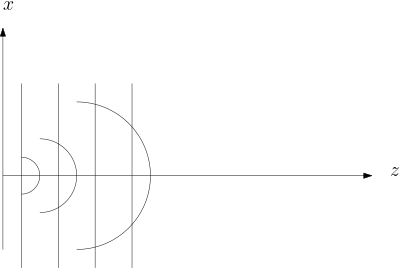
\includegraphics[height=2.0in]{figures/hw5/hw5_1.png}}
\caption{Propagating Spherical Wave and Planar Wave}
\label{fig:51}
\end{figure}

Assuming  no phase delay between the 2 waves, a plane waves $ou^{\prime}$ (what) axis propagating in $z$ can be written as 
$$g_{\mathrm{pw}}(x,z)=E_0 \exp \left \{ i \frac{2 \pi}{\lambda} z \right \}$$
where a spherical wave can be written as
$$g_{\mathrm{sw}}(x,z)= \frac{E_0}{i \lambda z} \exp \left \{ i \pi \frac{x^2}{\lambda z}  \right \} \exp \left \{ i \frac{2 \pi}{\lambda} z \right \}.$$
The interference pattern is given by the difference in phase of the 2 waves as a function of $x$ and $z$. Phase of the plane wave depends only on $z$
$$\phi_{\mathrm{pw}}(z)=\frac{2\pi}{\lambda}z$$
while the phase of the the spherical wave on both $x,z$.\\

In this regards, we will have in phase components when
$$\frac{\pi}{\lambda z}x^2 + \frac{3}{2}\pi = 2\pi m$$
which means when 
$$\Delta \phi = \phi_{pw} - \phi_{sw}$$
is an entire multiple of $2\pi$. We can solve for $x$ in Equation \ref{eq:51a1} and shown in Figure \ref{fig:51a02}.

\begin{equation}\label{eq:51a1}
\begin{array}{l}
\frac{\pi}{\lambda z}x^2 + \frac{3}{2}\pi = 2m \pi \\
x^2 = \left( 2m - \frac{3}{2} \right) \lambda z\\
m=1 \text{ \& } z=100\lambda \Rightarrow x = \pm \sqrt{\frac{1}{2}\lambda z} = \sqrt{\frac{1}{2}}10 \lambda\\
m=2 \text{ \& } z=100\lambda \Rightarrow x = \pm \sqrt{\frac{5}{2}\lambda z} = \sqrt{\frac{5}{2}}10 \lambda\\
\end{array}
\end{equation}

\begin{figure}
\centering\fbox{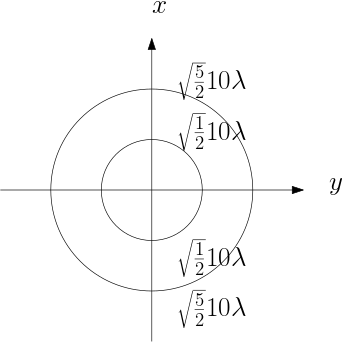
\includegraphics[height=2.0in]{figures/hw5/hw51a02.png}}
\caption{If we console the $y$ coordinate}
\label{fig:51a02}
\end{figure}

We can then solve 
$$\pi (x^2 + y^2) = (2m\pi - \frac{3}{2}\pi)\lambda z$$
which represents concentric rings of radii
$$radii = \sqrt{(2m - \frac{3}{2}) \lambda z}$$
where $\lambda z = 100 \lambda^2$

\item{Describe the interference pattern for an off-axis co-propagating plane wave ($\theta_1 = -30$ degrees and $\theta_2 = +45$ degrees in the xz plane with respect to z).}

We focus on the plane wave propagating with a $45\degree$ angle with respect to the $z$ axis in the $xz$ plane as shown in Figure \ref{fig:hw51b01}.

\begin{figure}
\centering\fbox{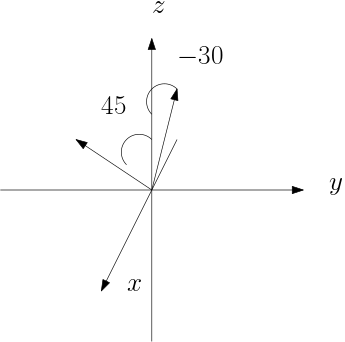
\includegraphics[height=2.0in]{figures/hw5/hw51b01.png}}
\caption{Axis Setup}
\label{fig:hw51b01}
\end{figure}

The plane wave can be written as 
$$g_{\mathrm{pw}}(x,z) = E_0 \exp \left(i (k_x x + k_z z) \right)$$
where $k_x$ and $k_y$ are the projections of the $k$ vector on the $x$ and $z$ axis.
$$k_x = k_0 \sin (45 \degree) = \frac{2 \pi}{\lambda} \frac{\sqrt{2}}{2} = \frac{\pi}{\lambda}\sqrt{2}$$
and
$$k_z = \frac{\pi}{\lambda}\sqrt{2}.$$

The phase difference between plane wave pw and plane wave sw in Equation \ref{eq:hw51b01}.

\begin{equation}\label{eq:hw51b01}
\begin{array}{l}
\phi_{\mathrm{pw}}(x,z)=\frac{\pi}{\lambda}\sqrt{2}(x+z)\\
\phi_{\mathrm{sw}}(x,z)=\frac{\pi}{\lambda z}x^2 + \frac{2\pi}{\lambda}z + \frac{3}{2}\pi\\
\Delta \phi = \frac{3}{2}\pi + \frac{\pi}{\lambda z}x^2 + \frac{2\pi}{\lambda}z - \frac{\pi \sqrt{2}}{\lambda}z - \frac{\pi \sqrt{2}}{\lambda}z
\end{array}
\end{equation}

The $z$ component solves to $\frac{\pi z}{\lambda}(2-\sqrt{2})$\\

Bright sports will be at $\Delta \phi = 2\pi m$ which is used to solve Equation \ref{eq:hw51b02} for the $x$ axis.

\begin{equation}\label{eq:hw51b02}
\begin{array}{l}
\frac{\pi}{\lambda z}x^2 - \frac{\pi}{\lambda}\sqrt{2}x + \frac{\pi z}{\lambda}(2-\sqrt{2}) - 2\pi m = 0\\
x^2 - \sqrt{2}zx + z^2(2-\sqrt{2}) - 2 m \lambda z = 0\\
x_{1/2}=\frac{\sqrt{2}z \pm \sqrt{2 z^2 + 4m \lambda z}}{2}
\end{array}
\end{equation}

\item{Is it possible to generate this kind of wave with a Michelson Interferometer?(Shown in Figure \ref{fig:53}) Please motivate and describe your answer extensively.}\\

Yes in order to obtain a spherical co propagate with a plane wave we can a convex lens in the measuring arm of an interferometer as shown in Figure \ref{fig:hw51c01}.\\

\begin{figure}
\centering\fbox{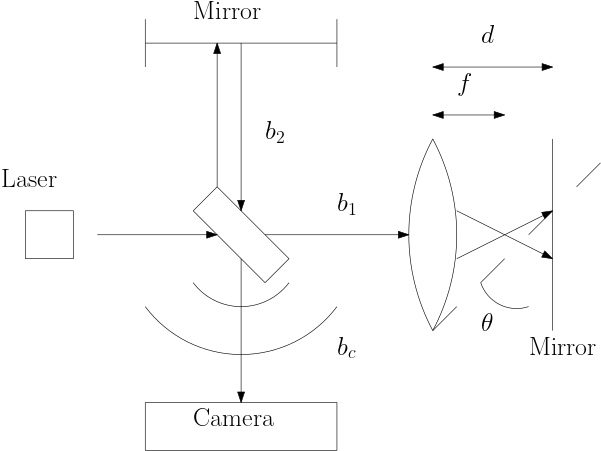
\includegraphics[height=2.0in]{figures/hw5/hw51c01.png}}
\caption{Michelson interferometer}
\label{fig:hw51c01}
\end{figure}

If $d=f$ we obtain again a plane wave in $b_c$. If $d \neq f$ we obtain the (???) of the spherical wave and a plane wave.

\end{enumerate}

% -----------------------------------------------------
% Ex 2 
% -----------------------------------------------------
\item{Consider a sinusoidal amplitude grating.}
$$g_t(x)=\frac{1}{2}\left[ 1+m\cos(\frac{2\pi x}{\Lambda} + \phi) \right]$$
at $z=0$. Illuminated by an off-axis plane wave.
$$g_{-}(x,z=0)=\exp(\frac{2\pi}{\Lambda}i \theta x)$$
\begin{enumerate}

\item{Derive the expression of $g_{\text{+}}(x,z=0)$}\\

For the amplitude grating, the geometry along the x-axis is considered because $z=0$. The Fresnel diffraction pattern, the field just behind the grating illuminated by the plane wave, shown in Figure \ref{fig:521} is defined in  Equation \ref{eq:521} where the phase shift $\phi$ is 0.

\begin{figure}
\centering\fbox{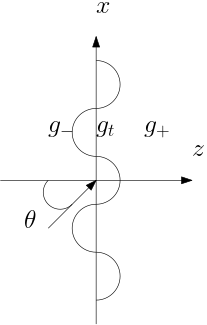
\includegraphics[height=2.0in]{figures/hw5/hw52a01.png}}
\caption{Sinusoidal amplitude grating}
\label{fig:521}
\end{figure}

\begin{equation}\label{eq:521}
\begin{split}
g_{+}(x, z=0) = \\
= g_{t}(x) g_{-}(x, z=0) \\
= \left [ \frac{1}{2} + \frac{m}{4} \left( \exp\left\{i \left( \frac{2\pi}{\Lambda}x + \phi \right) \right\} + \exp\left\{-i \left( \frac{2\pi}{\Lambda}x + \phi \right) \right\} \right) \right ] \cdot \exp \left( \frac{2\pi}{\lambda}i \theta x \right)\\
= \frac{1}{2} \exp \left( \frac{2\pi}{\lambda}i \theta x \right) + \frac{m}{4} \exp \left\{ i 2 \pi x \left(\frac{1}{\Lambda} + \frac{\theta}{\lambda} \right) \right\} + \frac{m}{4} \exp \left\{ -i 2 \pi x \left(\frac{1}{\Lambda} - \frac{\theta}{\lambda} \right) \right\}
\end{split}
\end{equation}

\item{What would be the interference pattern at infinity}

The interference pattern at infinity is given by the Fraunhofer diffraction, which is equal to the Fourier transform of the wave front in $z=0$ as shown in Equation \ref{eq:522}.

\begin{equation}\label{eq:522}
G_{out}= \int_{-\infty}^{\infty}g_{+}(x,z=0)\exp(-i 2 \pi u x)dx 
\end{equation}

Considering the translation properties of the Fourier transform $\int_{-\infty}^{\infty} \exp(i 2 \pi u_0 x)\exp(-i 2 \pi  u x)dz \Rightarrow \delta (u-u_0)$. The interference pattern is solved for in Equation \ref{eq:523} where $u=\frac{x^{\prime}}{\lambda z}$ and $u_{0} = \frac{\theta}{\lambda}$ and is shown in Figure \ref{fig:522}.

\begin{equation}\label{eq:523}
\begin{split}
G_{out} &= \frac{1}{2} \delta(u-\frac{\theta}{\lambda}) + \frac{m}{4} \delta(u - \left(\frac{1}{\Lambda} + \frac{\theta}{\lambda} \right)) + \frac{m}{4} \delta(u + \left(\frac{1}{\Lambda} - \frac{\theta}{\lambda} \right))\\
&= \frac{1}{2} \delta(u - u_0) + \frac{m}{4} \delta(u - u_0 - \frac{1}{\Lambda}) + \frac{m}{4} \delta(u - u_0 + \frac{1}{\Lambda}) 
\end{split}
\end{equation}
\end{enumerate}

\begin{figure}
\centering\fbox{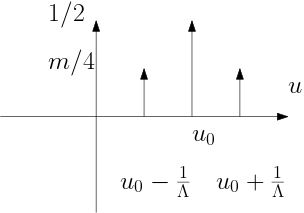
\includegraphics[height=2.0in]{figures/hw5/hw52b01.png}}
\caption{Interference Pattern at Infinity}
\label{fig:522}
\end{figure}

% -----------------------------------------------------
% Ex 3 
% -----------------------------------------------------
\item{Derive the interference pattern of a plane wave passing through a double split for $D=10\lambda$. Use Huygens' principle and derive the superposition of the waves at a distance $z=L$.}\\

Huygens principle states that each point on the wave front acts as a secondary light source emitting a spherical wave. The wave front after a short propagation distance is the result of superimposing all these spherical waves, adding the corresponding phasors including the phase delay incurred due to propagation.

\begin{figure}
\centering\fbox{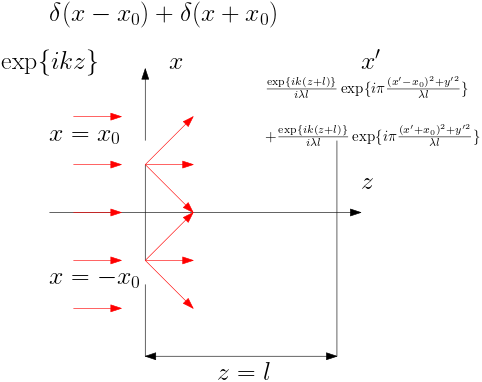
\includegraphics[width=4.0in]{figures/hw5/hw5q3.png}}
\caption{Two holes in an opaque screen with incoming plane wave on-axis}
\label{fig:53}
\end{figure}

Considering Huygenes principle, each aperture generates a spherical wave outward at $x-5\lambda$ and $x+5\lambda$. Alternatively we can consider the double slit as an optical transparency with two infinitesimally small aperture as shown in Equation \ref{eq:531} immediately after the double slit..

\begin{equation}\label{eq:531}
\begin{split}
g_t(x) = \delta(x-5\lambda) + \delta(x+5\lambda)\\
g_{-}(x) = \exp(i\frac{2\pi}{\lambda}z) \rightarrow \text{ at } z=0 \rightarrow g_{-}(x)=1\\
\therefore
g_{+}(x) = \delta(x-5\lambda) + \delta(x+5\lambda)
\end{split}
\end{equation}

According to the Fresnel integral,  the superposition of the waves at distance $z=L$ is defined in Equation \ref{eq:532} where the component inside the integral represents a convolution of a spherical wave and 2 $\delta$ functions. We also need to recall that in general a convolution between a $\delta$ and a function $f$ is $\delta(x-x_0) \ast f(x) = \int \delta(x-x_0)f(x^{\prime} -x)dx = f(x^{\prime}-x_0)$

\begin{equation}\label{eq:532}
\begin{split}
g_{out}(x^{\prime},z=L) = g^{\prime}(z=L) \int_{-\infty}^{\infty} g_t(x)\exp(\frac{i\pi(x^{\prime}-x)^2}{\lambda z})dx\\
= \frac{1}{i \lambda z}\exp\left\{ i 2\pi \frac{z}{\lambda} \right\} \int_{-\infty}^{\infty} g_t(x)\exp(\frac{i\pi(x^{\prime}-x)^2}{\lambda z})dx\\
= \frac{1}{i \lambda L}\exp\left( i 2\pi \frac{z}{\lambda} \right) \left\{ \exp(\frac{i\pi(x^{\prime}-5 \lambda)^2}{\lambda L}) + \exp(\frac{i\pi(x^{\prime}+5\lambda)^2}{\lambda L}) \right\}
\end{split}
\end{equation}

\end{enumerate}

\end{enumerate}
\end{document}